\PassOptionsToPackage{unicode=true}{hyperref} % options for packages loaded elsewhere
\PassOptionsToPackage{hyphens}{url}
%
\documentclass[]{article}
\usepackage{lmodern}
\usepackage{amssymb,amsmath}
\usepackage{ifxetex,ifluatex}
\usepackage{fixltx2e} % provides \textsubscript
\ifnum 0\ifxetex 1\fi\ifluatex 1\fi=0 % if pdftex
  \usepackage[T1]{fontenc}
  \usepackage[utf8]{inputenc}
  \usepackage{textcomp} % provides euro and other symbols
\else % if luatex or xelatex
  \usepackage{unicode-math}
  \defaultfontfeatures{Ligatures=TeX,Scale=MatchLowercase}
\fi
% use upquote if available, for straight quotes in verbatim environments
\IfFileExists{upquote.sty}{\usepackage{upquote}}{}
% use microtype if available
\IfFileExists{microtype.sty}{%
\usepackage[]{microtype}
\UseMicrotypeSet[protrusion]{basicmath} % disable protrusion for tt fonts
}{}
\IfFileExists{parskip.sty}{%
\usepackage{parskip}
}{% else
\setlength{\parindent}{0pt}
\setlength{\parskip}{6pt plus 2pt minus 1pt}
}
\usepackage{hyperref}
\hypersetup{
            pdftitle={Themelio: a new paradigm for decentralizing the Internet},
            pdfauthor={Yuhao Dong},
            pdfborder={0 0 0},
            breaklinks=true}
\urlstyle{same}  % don't use monospace font for urls
\usepackage{graphicx,grffile}
\makeatletter
\def\maxwidth{\ifdim\Gin@nat@width>\linewidth\linewidth\else\Gin@nat@width\fi}
\def\maxheight{\ifdim\Gin@nat@height>\textheight\textheight\else\Gin@nat@height\fi}
\makeatother
% Scale images if necessary, so that they will not overflow the page
% margins by default, and it is still possible to overwrite the defaults
% using explicit options in \includegraphics[width, height, ...]{}
\setkeys{Gin}{width=\maxwidth,height=\maxheight,keepaspectratio}
\setlength{\emergencystretch}{3em}  % prevent overfull lines
\providecommand{\tightlist}{%
  \setlength{\itemsep}{0pt}\setlength{\parskip}{0pt}}
\setcounter{secnumdepth}{0}
% Redefines (sub)paragraphs to behave more like sections
\ifx\paragraph\undefined\else
\let\oldparagraph\paragraph
\renewcommand{\paragraph}[1]{\oldparagraph{#1}\mbox{}}
\fi
\ifx\subparagraph\undefined\else
\let\oldsubparagraph\subparagraph
\renewcommand{\subparagraph}[1]{\oldsubparagraph{#1}\mbox{}}
\fi

% set default figure placement to htbp
\makeatletter
\def\fps@figure{htbp}
\makeatother


\title{Themelio: a new paradigm for decentralizing the Internet}
\author{Yuhao Dong}
\date{}

\begin{document}
\maketitle

\hypertarget{themelio-a-stable-blockchain-for-an-unstable-world}{%
\section{Themelio: a stable blockchain for an unstable
world}\label{themelio-a-stable-blockchain-for-an-unstable-world}}

\hypertarget{introduction}{%
\subsection{Introduction}\label{introduction}}

\hypertarget{a-blockchain-revolution}{%
\subsubsection{A ``blockchain
revolution''?}\label{a-blockchain-revolution}}

\hypertarget{the-promise-of-blockchains}{%
\paragraph{The promise of
blockchains}\label{the-promise-of-blockchains}}

Trust on the Internet is a rare commodity. Participants are often
anonymous, and communication is inherently insecure. Everyone is at most
a few hundred milliseconds away from potential attackers.

Generally, to trust someone on the internet you either know them in real
life or depend on trusted third party intermediaries. However,
real-world knowledge is extremely rare on the Internet, while
intermediaries (such as certificate authorities, lookup servers, and
notaries) are almost always centralized institutions. Unfortunately,
central points of trust are often single points of failure. Compromised
root CAs lead to catastrophic meltdowns of the basic cryptography of the
encrypted Web {[}@prins2011diginotar{]}. Poisoned DNS servers enable
defacings of high-profile websites. Hacked update servers can instantly
distribute malware to enormous numbers of unsuspecting computers,
crippling critical systems {[}@richardson2017ransomware{]}.

Moreover, centralized control of the ``commanding heights'' of our
modern interconnected society lends a disproportionate amount of power
to a small oligarchy of service providers. This enables a wide range of
abuse with devastating real-world consequences. For instance,
centralized social media platforms insidiously manipulate and censor
user communication {[}@sunstein2018republic{]}. As another example,
governments build Orwellian surveillance systems like the prototype
Chinese ``social credit'' system {[}@wang11china{]} by aggregating
massive amounts of data from centralized sources.

In the face of these numerous perils of centralization on the Internet,
blockchains offer an attractive alternative. Public blockchains like
Bitcoin {[}@nakamoto2008bitcoin{]} and Ethereum {[}@wood2014ethereum{]}
are unforgeable, append-only ledgers accessible to all. They provide
secure, transparent, and permanent records of transactions while being
completely decentralized. Instead of relying on unaccountable
centralized entities, applications such as public key infrastructures,
document timestamping services, and electronic money can now use this
shared ledger to guarantee security. Blockchains promise a revolution to
end reliance on dangerously fragile central trusted entities.

\hypertarget{where-are-all-the-blockchain-apps}{%
\paragraph{Where are all the blockchain
apps?}\label{where-are-all-the-blockchain-apps}}

Yet despite all the hype of a blockchain revolution, almost no
production systems use public blockchains. Naming even a \emph{single}
user-facing application using a public blockchain is astonishingly
difficult --- except for, of course, cryptocurrency trading apps,
blockchain viewers, and other such blockchain-centered software. Why?

Simply put, this is because \emph{public blockchains are not good
enough}. Firstly, Nakamoto consensus --- the very innovation that gives
public blockchains their robust decentralized consensus --- saddles
users with onerous costs. Take Bitcoin as an example: users must
synchronize and store the blockchain's entire transaction history, which
is hundreds of gigabytes and growing. On top of that, users must wait
hours for a transaction to become irreversible when the network is a bit
slow.

Furthermore, public blockchains can be quite unreliable. Wildly
fluctuating cryptocurrency prices create unnecessary currency risk;
congestion leads to spikes in transaction fees; and network problems
cause long delays. None of these shortcomings are acceptable in modern
production systems. Finally, public blockchains by nature require
unanimous agreement on the blockchain protocol. Therefore, protocol
upgrades are almost always disruptive and contentious --- every tiny
change can shake the whole blockchain ecosystem. Nobody wants to build
applications on a foundation that threatens their products' basic
integrity with every update.

Unsurprisingly, blockchains have failed to truly revolutionize the
software industry. Instead, their impact is mostly limited to inspiring
a breed of centralized databases with the catchy label of ``private
blockchains''. Although private blockchains, like those based on
Hyperledger Fabric {[}@cachin2016architecture{]}, use append-only
distributed ledgers similar to those of public blockchains, they're
generally deployed within an environment isolated from public access,
such as across a corporate WAN or even inside a single datacenter.
Enterprise applications, such as supply-chain tracking or processing
business payments, have an especially strong tendency towards using
private blockchains.

Unlike their public counterparts, private blockchains promise
performance and reliability comparable with traditional databases. For
this reason, private blockchains have been adopted by a wide variety of
production systems, ranging from the SecureKey identity service
{[}@securekey{]} to Estonian government systems {[}@estonia{]}.
``Blockchain for business'' is currently almost synonymous to a
blockchain within a private, controlled environment.

However, private blockchains by definition give up much of the security,
transparency, and decentralization of public blockchains. The majority
of proposed deployments, such as those within a single datacenter,
almost entirely abandon the promised paradigm shift towards
decentralization. Because private blockchains sacrifice decentralization
in pursuit of maximal usability, they are useless in bringing about a
more decentralized Internet.

\hypertarget{whats-wrong-with-blockchains}{%
\subsubsection{What's wrong with
blockchains?}\label{whats-wrong-with-blockchains}}

\hypertarget{attempts-at-better-blockchains}{%
\paragraph{Attempts at better
blockchains}\label{attempts-at-better-blockchains}}

Many projects attempt to build better blockchains. However, a large
number of these propose something categorically different from trustless
public blockchains, thus losing sight of the essence of blockchains in
pursuit of optimization. Here are two examples.

One fairly obvious idea is to compromise between private and public
blockchains to get the best of both worlds. ``Consortium'' blockchains
--- blockchains where participation is limited to a small number of
trusted partners --- are a good example. This includes Quorum
{[}@quorum{]}, an Ethereum-based consortium blockchain designed to be
deployed in enterprise backend services and Corda {[}@corda{]}, which is
designed to provide business-to-business secure transactions. Consortium
blockchains may also support public access, though not universal
participation in the consensus protocol. Some blockchains, like EOS,
even elect the consortium from the wider public.

Limiting the number of consensus participants typically improves
performance and reliability simply because the data needs to be
replicated dramatically fewer times (this is the the same reason why
private blockchains are superior in these aspects). Unfortunately,
``hybrid'' blockchains retain most of the problems of either public or
private blockchains. Those that deliver reliable performance and agile
updates end up with the poor security and inadequate decentralization of
private blockchains. Others that emphasize security inherit the poor
performance and inflexibility of public blockchains. Ultimately,
retaining decentralized trust requires wide-scale consensus, while
reducing the overhead of consensus necessarily translates into
diminished security and neutrality.

A second approach is altogether abandoning the model of a unified,
trustless append-only log. This includes ``sharded'' designs for
blockchains, such as Omniledger {[}@kokoris2018omniledger{]}, and
non-blockchain ledgers like Ripple {[}@armknecht2015ripple{]} and
Hashgraph {[}@baird2016swirlds{]}. Though forgoing the requirement for a
universally replicated log eliminates most scalability challenges, it
introduces far greater complexity in both the implementation and
application interfaces. This only exacerbates the already daunting
difficulty in developing applications on blockchains. In fact, none of
these ``unconventional'' distributed ledgers have achieved much
production success. After all, distributed consensus protocols have
existed for decades. It is precisely the simple yet expressive
abstraction of a linear blockchain that has fascinated the world, yet
unconventional ``blockchains'' have chosen to throw it away.

\hypertarget{are-blockchains-stuck}{%
\paragraph{Are blockchains stuck?}\label{are-blockchains-stuck}}

The very existence of multiple ``non-blockchain'' attempts to fix
blockchains hints that public blockchains as conventionally conceived
have fundmental problems. Indeed, current blockchains encounter three
significant problem areas:

\begin{enumerate}
\def\labelenumi{\arabic{enumi}.}
\tightlist
\item
  \textbf{Horizontal scalability}: Global replication and consensus,
  which are fundamental to the desired blockchain properties, pose
  severe information-theoretical limits on scaling horizontally.
  Decentralized apps running on blockchains are already running into
  this problem, which manifests as expensive and variable fees and poor
  reliability. In fact, even private and consortium blockchains
  typically cannot compete with the performance of traditional
  centralized services.
\item
  \textbf{Governance}: Implementing protocol changes in public
  blockchains has proven to be fiendishly difficult ``political''
  decisions. They involve much controversy and fail to come to
  satisfactory results even for simple changes like that of Bitcoin's
  block size limit.
\item
  \textbf{Usability}: Blockchains tend to be ``leaky'' abstractions,
  requiring developers of blockchain applications to understand
  low-level details such as block reorganizations and transaction fee
  auctions. This causes usability problems throughout blockchain
  applications and often forces end users to deal with the blockchain's
  technical problems.
\end{enumerate}

All three problems appear somewhat inherent to the blockchain design and
therefore difficult to remedy. Distributed consensus is by nature hard
to scale; permissionless blockchains do not have any authority that can
``govern'' the protocol; blockchains have peculiar characteristics, like
Nakamoto consensus, that make usable abstractions hard to build.

Much work has already been done on incrementally attacking these
daunting problems, but the issues cannot be wholly eliminated by
localized optimization. These problems are symptoms of a more
fundamental issue in the very way blockchains are used and designed.

\hypertarget{the-crux-endogenous-trust}{%
\paragraph{The crux: endogenous trust}\label{the-crux-endogenous-trust}}

We cannot build a better blockchain without understanding what exactly
makes blockchains unique. Despite their popularity, many of blockchains'
widely-touted features are also found in other systems. For example,
\emph{decentralization} is often proclaimed as a key asset of
blockchains, but many existing systems have decentralized governance
without a central trusted party. This includes DHTs, email, the PGP web
of trust, and even the Internet itself. \emph{Transparency} is another
commonly-cited advantage of blockchains, yet many non-blockchain
protocols like Certificate Transparency and Keybase also use
transparency as a key part of their security. Thus, neither
decentralization nor transparency constitute the essence of blockchains.

Instead, the crucial feature that distinguishes blockchains from all
preexisting protocols is \textbf{endogenous trust}. That is, we can
trust that a blockchain protocol will behave in a certain way with
\emph{minimal assumptions about who runs it}. In blockchains, trust
emerges from \emph{within} the protocol, not from preexisting trust in
the parties that run the protocol. Crucial to endogenous trust is
\emph{cryptoeconomics}, the intersection of game theory and cryptography
that enables the formal design of self-incentivizing mechanisms so that
given enough participants, we can trust the group's overall behavior
without trusting any individual participant.

Endogenous trust is the single most precious property of blockchains
that enables secure applications with properties elusive to
pre-blockchain systems. For example, someone using a bank must trust the
bank no matter what form of communication protocol is used, yet a
Bitcoin user does not need to even know which miner ends up processing
their transaction, let alone establish some sort of trust with that
miner. Instead, the cryptoeconomics of Bitcoin mining internally
incentivize miners to cooperate in such a way that makes the Bitcoin
protocol as a whole trustworthy.

Many blockchain failures can, in fact, be analyzed as failures in
endogenous trust. Contentious governance problems like the Bitcoin
block-size controversy of 2017 or the ``DAO fork'' that split Ethereum
into Ethereum and Ethereum Classic arise when external factors
incentivize users to override a blockchain's endogenous trust mechanism.
Poor internal incentives cause out-of-band coordination to become
necessary to prevent game-theoretical issues like ``SPV mining'' in
Bitcoin. Even volatile cryptocurrency prices can be analyzed as a lack
of an endogenously trustworthy store of value, forcing users to reach
for fiat-pegged stablecoins like Tether that altogether forgo endogenous
trust.

Regretfully, the frequency of failure reveals that, in reality,
endogenous trust in blockchains is very fragile and often subverted,
despite it being the soul of blockchains. Why is that so? An inspection
of the state of the art in blockchains reveals the reason.

\hypertarget{weak-endogenous-trust-in-existing-blockchains}{%
\paragraph{Weak endogenous trust in existing
blockchains}\label{weak-endogenous-trust-in-existing-blockchains}}

Blockchains nowadays can be roughly divided into two categories:

\begin{itemize}
\tightlist
\item
  \textbf{Application blockchains} are optimized for one particular
  application. They often have adequate usability and performance at the
  expense of adaptability to diverse usages. Examples include Bitcoin
  Cash (higher throughput bitcoin), Filecoin (incentivized peer-to-peer
  content distribution), and Zcash (untraceable payments).
\item
  \textbf{Platform blockchains} attempt to provide the full set of
  features needed to implement decentralized applications, typically
  through Turing-complete ``smart contracts''. Ethereum is the
  archetypal Swiss army knife blockchain; newer examples include EOS and
  Tezos.
\end{itemize}

Yet both kinds of blockchains fail at providing strong endogenous trust.
This is due to two common problems.

First, \emph{weak cryptoeconomics} often undermine incentive structures
intended to secure the blockchain endogenously and force the community
to resort to out-of-band coordination to keep the ledger secure.
Unpredictable social processes such as Bitcoin's coordination
surrounding SPV mining and EOS's node elections all result from a lack
of built-in incentives nudging participants towards secure behavior.
Both application and platform blockchains suffer from poorly designed
cryptoeconomic incentives, especially the latter due to their more
complex protocols.

The second, and perhaps more important, cause of poor endogenous trust
is \emph{application-blockchain friction}. Application-blockchain
friction occurs when a blockchain protocol becomes increasingly
unsuitable for its main application. When this happens, the blockchain
loses its users' confidence. This forces a contentious out-of-band
protocol upgrade to prevent the blockchain from passing into the dustbin
of history. The Bitcoin block-size controversy is the most well-known
case of loss of trust from application-blockchain friction ---
unsurprising given Bitcoin's rigid coupling of its core payment
application to its blockchain.

Unfortunately, general-purpose blockchains like Ethereum experience even
more challenges to their endogenous trust due to application-blockchain
friction. In fact, as we have seen in the previous section, most of the
protocol upgrades to Ethereum so far involved fairly minor tweaks to
functionality in order to support newly emerging, unanticipated
applications.

The prevalence of application-blockchain friction is because both
application blockchains (like Bitcoin) and platform blockchains (such as
Ethereum) are \emph{are on the wrong protocol layer}. Both are \emph{too
close to applications}.

Platform blockchains like Ethereum sit directly underneath applications
to allow apps' easy deployment --- a new cryptocurrency can be
implemented on Ethereum in a few dozen lines of code. Such a direct
interface between application and blockchain, however, inevitably
results in contention between ever-changing application requirements and
ideally immutable blockchain protocols. The situation is analogous to
telecommunication networks before the Internet, where a vertically
integrated system directly offered relatively high-level functions like
voice calling and teletype. Like Ethereum, these complex platforms were
extremely costly to upgrade when they were forced to change by the rise
of new applications and technological advances.

Learning from previous these mistakes, it is clear that a blockchain
with endogenous trust must be built upon a solid cryptoeconomic
foundation. This ensures that its core security properties will require
no out-of-band social coordination to uphold. More importantly, it must
also minimize application-blockchain friction by using a protocol
analagous to the Internet Protocol --- a minimal, low-level protocol
with straightforward semantics. This allows easily upgradable
``middleware'' protocols to separate the blockchain from the
ever-changing needs of applications. Thus, the blockchain can remain an
embedded ``endogenous trust engine'' for decades without changing.

\hypertarget{towards-a-new-paradigm}{%
\subsubsection{Towards a new paradigm}\label{towards-a-new-paradigm}}

\hypertarget{a-minimal-blockchain}{%
\paragraph{A minimal blockchain}\label{a-minimal-blockchain}}

This points us towards a new blockchain paradigm --- a \emph{minimal
blockchain} acting as a bare-bones root-of-trust infrastructure for
supporting endogenoust rust in decentralized applications. Essentially
all other concerns would be subordinated to these two goals.

Current blockchains, as a matter of fact, are very far from the ideal
root of trust. Thus, a minimal blockchain design needs to sharply
diverge with existing blockchains in the following ways:

\begin{itemize}
\tightlist
\item
  \textbf{Minimal governance}: The protocol should be as simple and
  robust as possible to simply obviate the need for ongoing protocol
  changes. Deeply embedded infrastructure, such as the Internet
  Protocol, tend to only be useful if reasonably ``timeless''. This is
  essentially a stronger version of ``Szabo's Law'' (``blockchains
  should not be changed for non-technical reasons''), extended even to
  technical concerns. Current blockchains, on the other hand, regularly
  introduce consensus-breaking protocol changes, especially complex
  platform blockchains like Ethereum.
\item
  \textbf{Vertical scalability}: We intentionally avoid pursuing
  sharding and other horizontal scaling strategies, as they inherently
  violate logical centralization due to the CAP theorem
  {[}@brewer2012cap{]}. Instead, we want a blockchain that effortlessly
  scales throughput with increasing per-node computational capacity,
  while supporting fully secure ``thin'' clients and layer-2 strategies
  such as state channels at essentially indefinite scale. This is in
  sharp contrast to present blockchains, where ever-more-subtle shades
  of eventual consistency are used to support horizontal scaling,
  protocols treat thin clients as second-class citizens, and most
  applications are embedded directly in the blockchain state.
\item
  \textbf{Cryptoeconomic robustness}: To maximize endogenous trust, we
  want a blockchain designed with conservative cryptoeconomic
  assumptions that work without intervention in a wide variety of
  environments. This is, again, often neglected in current blockchain
  designs, especially newer projects focused on the putative
  scalability, governance, or usability issues.
\item
  \textbf{Simple abstractions}: Finally, we always choose simple,
  easy-to-understand abstractions over potentially more powerful but
  ``leakier'' ones. For example, we certainly wish to avoid the highly
  counterintuitive behavior of Nakamoto consensus.
\end{itemize}

All of these goals attack \emph{systemically infectious} problems in
current blockchains when used as a root of trust. No amount of
intervening abstraction can protect applications and end users from
interventionist governance, sharding-related data inconsistency,
cryptoeconomic attacks, and leaky abstractions, all of which can be
traced to the application/platform dichotomy and poor endogenous trust.
On the other hand, a minimal blockchain that aggressively attacks these
systemic problems allows easy encapsulation with well-designed
abstractions that hide technical details.

A minimal blockchain, rather than looking like an application or
platform, takes inspiration from the technology underpinning most of
modern telecommunication: the Internet Protocol (IP). IP gets packets on
a best-effort basis from point A to point B, and nothing more.
Unreliable datagrams don't make a developer-friendly interface, but they
do provide a firm foundation for ever-changing application protocol
stacks. IP is a great illustration of a successful foundational
technology. Such protocols are often too simple to support rich
applications without intervening protocol stacks, but they are easy to
conceptualize, simple to implement, and brutally robust. It is precisely
this simplicity that allows it to support the dazzling variety of
Internet applications today with practically no changes since the IPv4
specification's publication in 1981.

\hypertarget{building-a-rich-ecosystem}{%
\paragraph{Building a rich ecosystem}\label{building-a-rich-ecosystem}}

One disadvantage of a minimal blockchain is that it would be difficult
to use directly, as it would lack many features developers take for
granted, such as a powerful smart-contract system. A minimal blockchain
only makes sense within the context of a richly layered ecosystem, with
many abstraction tools available to application developers. Unlike a
monolithic platform blockchain, such an ecosystem would be able to
rapidly evolve without compromising the blockchain's immutability.

A decentralized-trust ecosystem of applications in this new model can
roughly be divided into three layers:

\begin{itemize}
\tightlist
\item
  \textbf{Themelio}, a minimal blockchain providing endogenous trust to
  the entire ecosystem
\item
  \textbf{Themelio standard protocols} providing standardization for
  ``middleware'' constructs such as state channels, a global naming
  system, etc that are not hard-coded into the blockchain and may evolve
  over time
\item
  \textbf{Applications} leveraging the Themelio infrastructure to
  achieve security and decentralization properties impossible without
  blockchains.
\end{itemize}

Themelio and its upper-layer protocols concretely instantiate the
concept of a minimal blockchain supporting a layered ecosystem. In the
process, we investigate and answer three important research questions
corresponding to the three divisions above:

\begin{itemize}
\tightlist
\item
  \emph{What is the optimal minimal blockchain?} It seems clear that
  blockchains should be pushed further away from the application, but
  what should be the division of functionality between the blockchain
  and upper-layer protocols? Simply removing ``messy'' features from
  existing blockchains will not do, as their entire architecture has not
  been designed with our paradigm in mind. Exploration of this question
  has in fact motivated many innovative design choices in Themelio.
\item
  \emph{How to build a ``blockchain-minimizing'' trustless protocol
  suite?} Except for a few specific ``off-chain'' applications such as
  state channels and cross-chain transfers, research in
  algorithmic-trust (``trustless'') protocols have largely assumed a
  blockchain-embedded or similar environment with ubiquitous logical
  centralization. We need to design network protocols which use our
  minimal blockchain to provide critical security guarantee, yet
  ``live'' largely outside the blockchain to maximize scalability and
  flexibility.
\item
  \emph{What do applications in such a paradigm look like?} Finally, we
  explore specific user-facing applications built in this sort of
  paradigm. We will see that such applications can be exceptionally
  user-friendly and reliable compared to current blockchain-based
  applications, while avoiding the governance and security problems
  inherent with traditional centralized-trust apps.
\end{itemize}

\hypertarget{themelio-a-minimal-blockchain}{%
\subsection{Themelio: a minimal
blockchain}\label{themelio-a-minimal-blockchain}}

In this chapter, the details of Themelio are laid out. Instead of a
specific decentralized application or a ``Swiss army knife'' runtime
environment, Themelio provides a \emph{minimal root of trust}. Themelio
sits at the bottom of diverse evolving protocol stacks, providing a
foundation of endogenous trust and logically centralized consensus ---
but not much else.

But how are we to build such a blockchain? We combine an elegant,
time-tested application interface --- a ``coin-based'' transaction graph
like that of Bitcoin --- with numerous innovations under the hood.
Consensus, based on proof of stake, is immediate, scalable, and highly
secure. Cryptocurrency is issued in a completely decentralized manner,
yet remains immune to bubbles that destabilize the exchange rate. A
simple yet expressive scripting language allows developing advanced
decentralized apps without the problems associated with stateful smart
contracts. These are some of the many features we use to maximize
robustness and performance.

\hypertarget{design-goals}{%
\subsubsection{Design goals}\label{design-goals}}

Let's first examine what we want to accomplish, and what we don't.

\hypertarget{goals}{%
\paragraph{Goals}\label{goals}}

Our overarching goal leads us to design Themelio according to these
principles:

\begin{enumerate}
\def\labelenumi{\arabic{enumi}.}
\tightlist
\item
  \textbf{Simple abstractions}: Themelio should present simple,
  ``non-leaking'' abstractions. Programmers without much experience with
  blockchains should be able to easily understand the features and
  behavior of the Themelio blockchain. We try our very best to avoid
  forcing users to consider subtle edge cases. For example, we must
  avoid many blockchains' unintuitive behavior in the presence of
  network latency (``confirmations'', forks, reorganizations).
\item
  \textbf{Stable protocol}: An initial period of rapid evolution is
  inevitable. But once mature, Themelio's internals should change as
  little as possible. Protocol stability avoids dangerous and messy
  consensus-breaking updates. Even though many blockchains envision
  constant protocol evolution, this introduces difficult out-of-band
  coordination problems --- otherwise known as politics. This can easily
  lead to de-facto centralization, contentious forks, and subversion by
  special interests. In Themelio, consensus-breaking changes will be
  made only in exceptional, non-controversial circumstances, such as to
  fix critical security vulnerabilities.
\item
  \textbf{Currency stability}: Themelio's cryptocurrency, the mel, is
  designed to have very low price volatility. It avoids large price
  increases, even with spikes in demand. The mel is designed to be a
  good unit of account and store of value, not a speculative asset
  exciting to ``HODL'' (``hold on for dear life'').
\item
  \textbf{High performance}: Themelio's performance must be much higher
  than existing public blockchains. This means both high transaction
  throughput and scalability in the number of fully secure clients.
  Decentralized apps with debilitatingly poor performance cannot take
  over the world.
\item
  \textbf{Application neutrality}: Themelio should not attempt to
  prevent or censor any categories of applications. It does not have an
  ``intended use''.
\item
  \textbf{Robust decentralization}: The ideal public blockchain must
  simulate a universally trusted intermediary --- decentralization is a
  must. Themelio is designed to decentralize trust across as large a
  population of stakeholders as possible. No unaccountable third
  parties, including network operators, should be able to subvert its
  security guarantees.
\end{enumerate}

\hypertarget{a-robust-transaction-model}{%
\subsubsection{A robust transaction
model}\label{a-robust-transaction-model}}

We start with a conceptual exploration of Themelio's high-level
transaction model: the abstractions on the blockchain that applications
interact with.

\hypertarget{coin-based-transactions}{%
\paragraph{Coin-based transactions}\label{coin-based-transactions}}

Themelio's basic transaction model belongs to a family usually known as
``UTXO-based'' or ``coin-based'' models. This is the oldest family of
blockchain models, including first-generation blockchains like Bitcoin
and Litecoin. In a coin-based model, the blockchain can be understood as
a grow-only directed acyclic graph (DAG) of \emph{transactions}. Every
transaction on the blockchain takes as input and spends one or more
\emph{unspent transaction outputs (UTXOs)} of previous transactions,
which are informally known as \emph{coins}. It then produces as output
one or more coins that can be spent as input by subsequent transactions.

Every coin represents a given amount of cryptocurrency, known as its
\emph{value}, and it includes an \emph{unlock constraint} that specifies
what sort of transaction can spend the coin. Each coin can only be spent
once. Excepting transactions that ``mine'' more currency, the sum of the
values of all the coins spent by a transaction must equal the sum of the
values of all the coins created by it.

Let's illustrate how coin-based transactions work with a simple example.
Assume there are 5 coins identified as \(B_1,\dots,B_{5}\), each worth
\$1, and each having an unlock constraint specifying ``any transaction
that spends me must have Bob's signature''. Informally, we say that Bob
owns 5 coins, each one worth \$1. Bob ``owning'' a coin simply means Bob
knowing how to satisfy the coin's unlock constraint.

Now, assume that Bob wants to send his friend Alice \$2.5. He creates a
new transaction spending \$\(B_1,B_2,B_3\)\$ as input, with two outputs:

\begin{itemize}
\tightlist
\item
  \[A_1\] with value \$2.5 and a constraint requiring Alice's signature.
\item
  \[B_6\] with value \$0.5 and a constraint requiring Bob's signature.
\end{itemize}

and informs Alice about \[A_1\]. Bob now ``owns'' \[B_4,B_5,B_6\] with a
total value of \$2.5, and Alice owns \[A_1\] with a total value of
\$2.5, just as we wanted. Note that Bob had to give himself a new coin
for the transaction to balance; this new coin is known as a \emph{change
output}. This picture from bitcoin.org shows a complex series of
interdependent coin-based transactions:

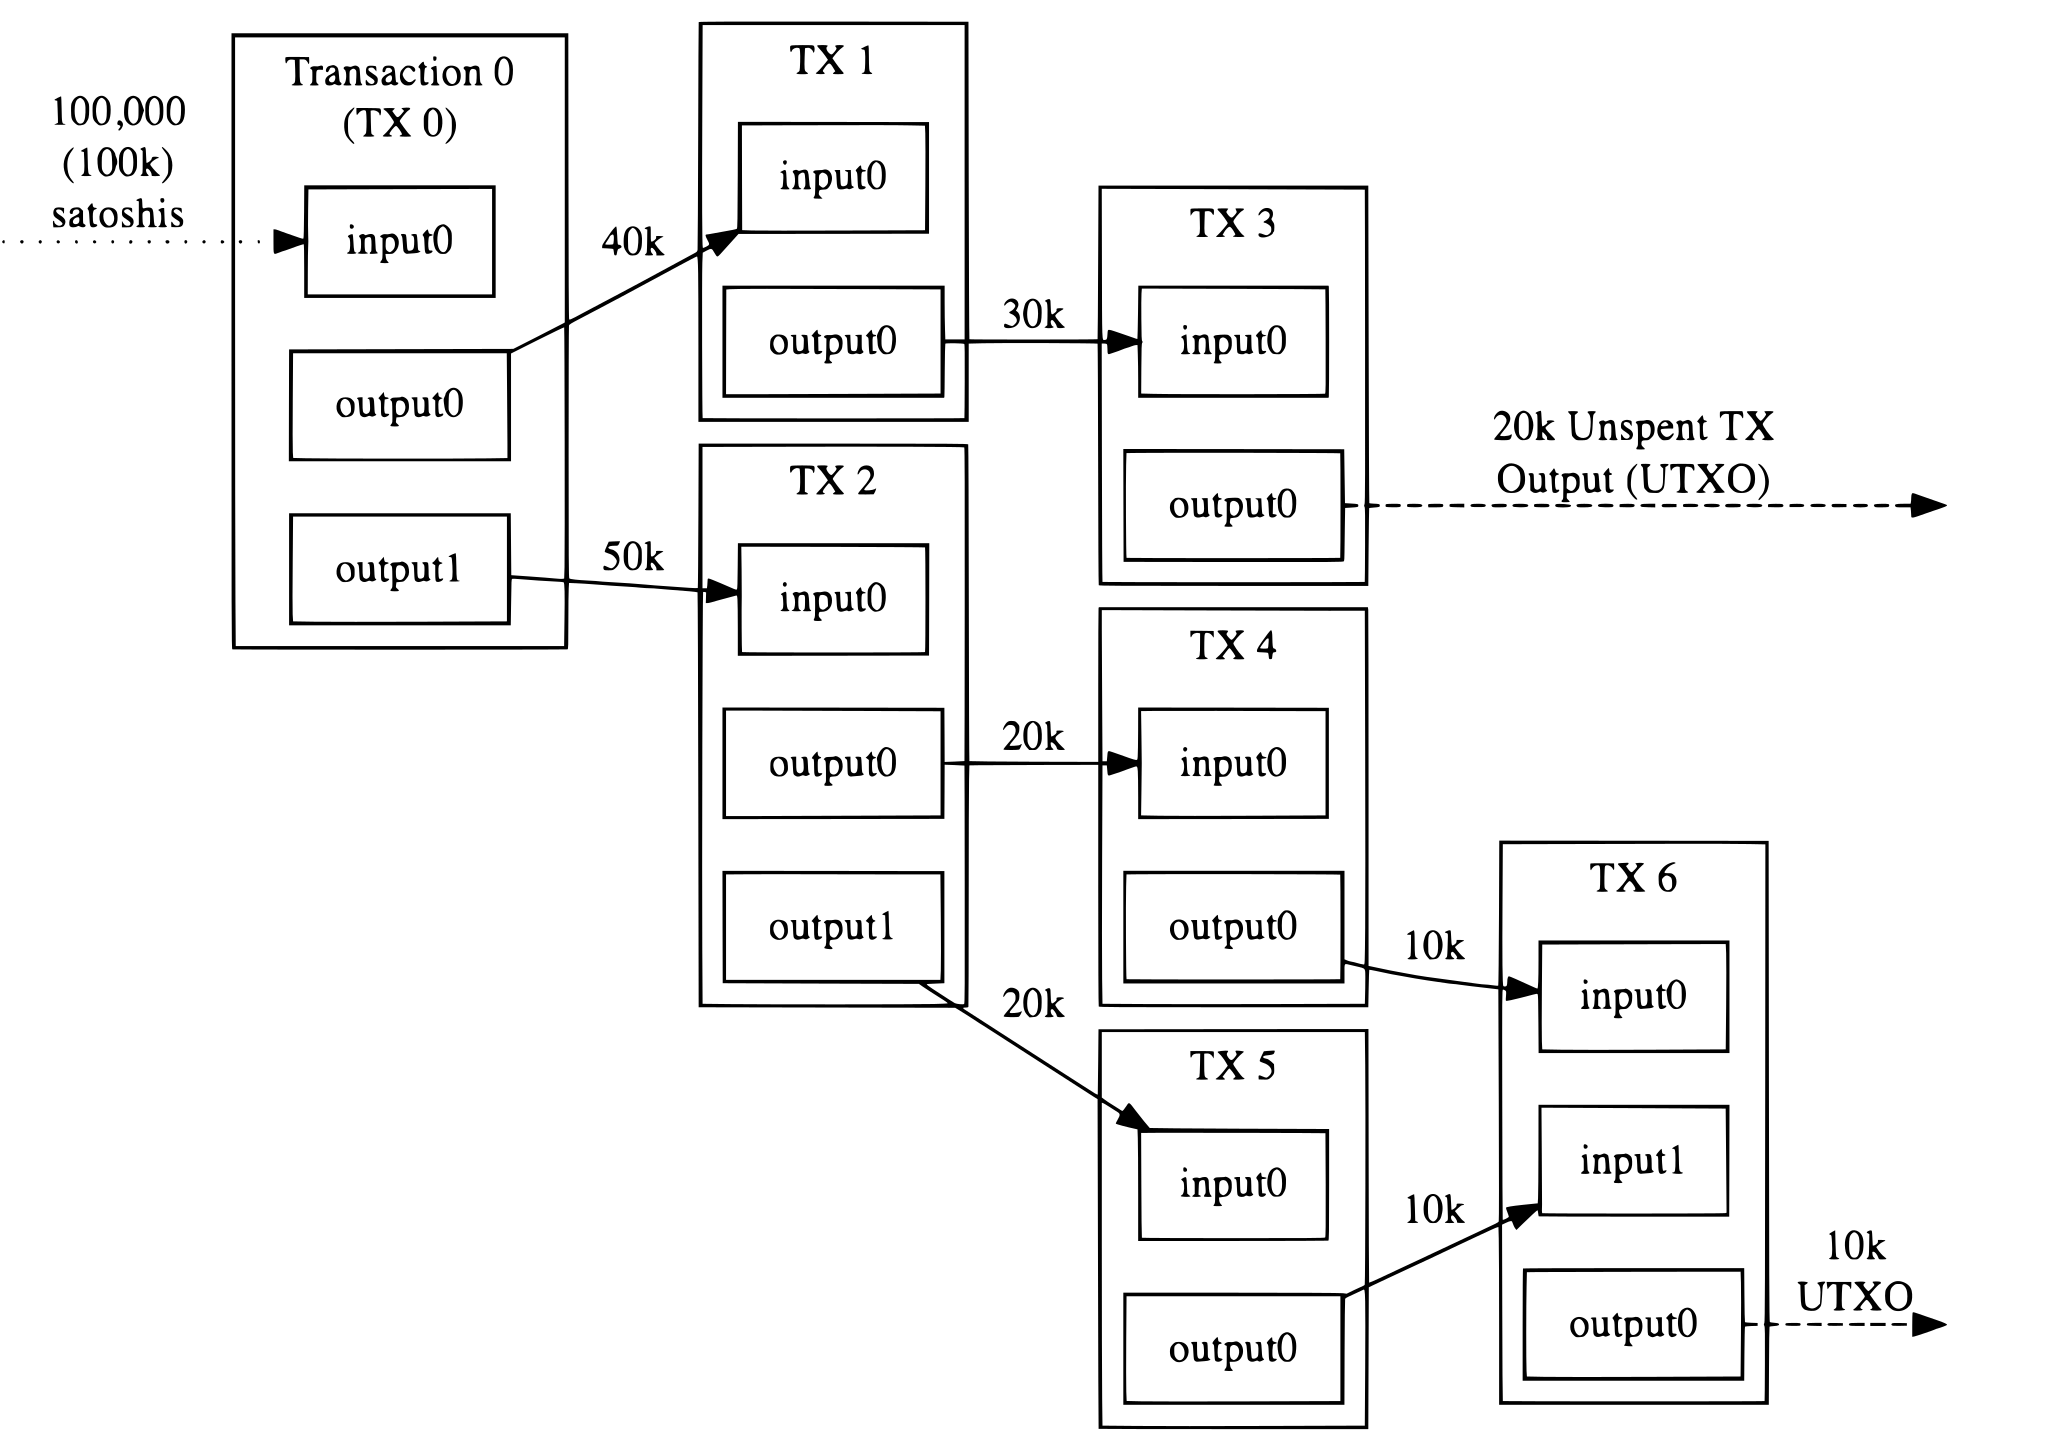
\includegraphics{../.gitbook/assets/utxo.svg}

Transactions are batched into an ever-growing series of \emph{blocks},
each one containing transactions settled in a particular time period.
Transactions within a block have no defined order --- the block that a
transaction belongs to is the smallest unit of time on the blockchain.
Finally, blocks are guaranteed to be \emph{consistent} , so all users of
the blockchain see the same blocks and the same transaction DAG.

\hypertarget{why-coins}{%
\paragraph{Why coins?}\label{why-coins}}

In Themelio, we use coin-based transactions with a cryptocurrency that
we call the \emph{mel}. We believe that a model of interdependent
transactions spending and producing coins, though originally invented
only for modeling money transfers, is a very good abstraction on which
decentralized-trust applications can be built.

But coin-based models are not popular at all among general-purpose
blockchains. Most blockchains attempting to support general
decentralized apps use \emph{account and smart-contract} based models.
In these models, accounts directly map to sums of money that can be
transferred and accounts can have automatically executing code attached.
In fact, the only general-purpose blockchain we know of that uses a
coin-based model is Qtum. Even there, an ``Account Abstraction Layer''
simulates Ethereum-like accounts to run smart contracts. Why do we
believe coins are the way to go?

First of all, coins allow Themelio to \textbf{process transactions
quickly}. In an account-based model, like in Ethereum or traditional
banking, strict global transaction ordering is necessary. Yet coin-based
transactions can be processed in any topological order --- we simply
need to process the transaction that produces a coin before the
transaction that spends it. Transactions within a block can be validated
mostly in parallel. This greatly increases performance.

Secondly, a coin-based architecture \textbf{simplifies state
transitions}. Blockchain protocols can be thought of as state-transition
functions, where each transaction takes in the ``world'' in a certain
state (say, Bob having \$5 and Alice \$0) and outputs a different state
(Alice and Bob both having \$2.5). To support functionality beyond basic
payments, account-based blockchains like Ethereum need arbitrarily
mutable global state, accessed by user-programmable ``smart contracts''.
However, programming decentralized apps with mutable state is
notoriously prone to error. Complex state transitions are associated
with difficult-to-find bugs and blockchain-level performance problems.
In a coin-based blockchain, state is extremely simple: the set of all
unspent coins. All transitions simply correspond to individual
transactions deleting and adding coins atomically. This leads to clearer
logic in decentralized apps and faster performance.

Finally, coin-based transactions are \textbf{surprisingly expressive}. A
very large class of security-critical problems boil down to establishing
a consistent, valid graph of interdependent events. For example, in a
naming system, a successful name transfer depends on previous events
like the previous owner relinquishing control, that owner first
registering the name, and so forth. Centralized roots of trust, like
notaries, certificate authorities, and banks, almost always serve the
role of ensuring consistency of an event graph. In a coin-based
blockchain model, the transaction DAG maps extremely well to these event
graphs. This means it's easy to write decentralized apps that replicate
centralized authorities on Themelio's coin-based model.

However, traditional coin-based architectures exactly like Bitcoin
clearly cannot support a wide variety of decentralized apps. Otherwise,
why would anybody use other blockchains? Themelio refines the
traditional coin-based model with two significant changes:
\emph{expressive constraint scripting} and a \emph{coin-oriented
application interface}. The former allows programs representing far more
than mere ``ownership'' to constrain coin spending. The latter makes it
much easier to write high-performance decentralized apps. Let's now
examine these two innovative features of Themelio's transaction model.

\hypertarget{constraint-scripting-with-melscript}{%
\paragraph{Constraint scripting with MelScript
}\label{constraint-scripting-with-melscript}}

Themelio allows users to write very complex unlock constraints with a
powerful scripting language, MelScript. Unlike Bitcoin unlock scripts,
MelScript can place conditions on any part of the transaction attempting
to spend a coin and enables easy development of a wide variety of
decentralized apps. Yet unlike Ethereum's EVM, MelScript is
Turing-incomplete and has no access to persistent state, eliminating a
large class of ``smart contract'' bugs.

MelScript is written in a Lisp-like syntax and compiled to a stack-based
bytecode to be embedded in transaction outputs. Simple, Bitcoin-like
constraints are straightforward. For example, the following is MelScript
for a ``multisignature'' constraint, for coins requiring signatures from
both \texttt{ALICE-KEY} and \texttt{BOB-KEY} to be spent:

\begin{verbatim}
(and (sig-correct? ALICE-KEY)
     (sig-correct? BOB-KEY))
\end{verbatim}

We can also access certain facts about the blockchain external to the
transaction attempting to spend a coin. For example, the following
constraint, which can't be expressed in Bitcoin's simplistic constraint
language, gives ownership of a coin to Alice if the total number of
transactions exceeds a million before the 10,000th block, and Bob
otherwise. It can be used as a simple bet between Alice and Bob on
Themelio's future adoption:

\begin{verbatim}
(if (and (> (get-stat 'transaction-count) 1000000)
         (< (get-stat 'block-height) 10000))
    (sig-correct? ALICE-KEY)
    (sig-correct? BOB-KEY))
\end{verbatim}

The most useful constraints in MelScript are not the simple filters
demonstrated above, but constraints that constrain constraints. This
allows us to embed a wide variety of decentralized, permissionless
secure data structures within the transaction graph, which we might call
\emph{coin structures}.

This is confusing, so let's illustrate the concept with an example.
Catena {[}@tomescu2017catena{]} is an append-only log originally
implemented in Bitcoin. The basic idea is simple: a central authority
can transparently publish a log of messages by building a transaction
chain, each spending the first output coin of the previous transaction.
Since coins cannot be spent twice, the authority cannot rewrite,
reorder, or delete any log entries after they are published. Here's an
illustration of a Catena log:

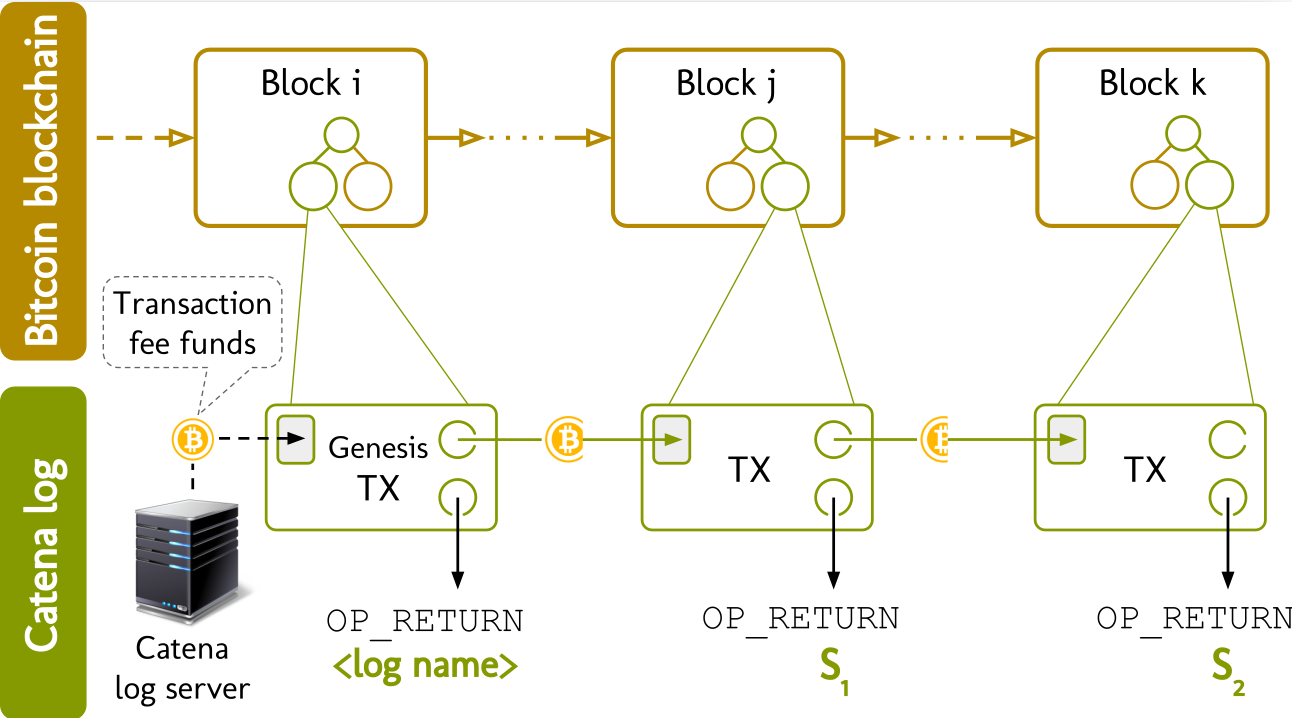
\includegraphics{../.gitbook/assets/screenshot-from-2020-08-27-17-14-00.png}

In Bitcoin and other existing coin-based blockchains, Catena logs must
be maintained by central authorities. Coins forming the chain must be
``owned'' by the log publisher, lest someone spend them for other
purposes and ruin the log. This prevents the use of Catena in
applications without a central publisher. In Themelio, however, we can
easily write a MelScript constraint that only allows transactions that
grow the Catena chain to spend the coin. Any coin with the following
constraint is forced to be the start of a permissionless Catena chain
that can never be broken:

\begin{verbatim}
;; at least 1 output coin
;; first output constrained the same way
;; *SELF* is the coin in which this constraint is embedded
(and (> (output-count) 0)
     (eq? (output-constraint (output-ref 0))
          (output-constraint *SELF*)))
\end{verbatim}

Coin structures, of course, are not limited to simple logs. Bitforest
{[}@dong2018bitforest{]} builds an entire naming system out of a coin
structure that implements an equivocation-proof binary search tree, yet
like Catena it must rely on a centralized coin owner when deployed on
existing blockchains. Analogous MelScript constraints can be used to
implement Bitforest on Themelio as an entirely decentralized and
permissionless naming system, with features comparable to naming systems
on ``smart contract'' blockchains, like the Ethereum Naming System
(ENS).

\hypertarget{coin-oriented-interface}{%
\paragraph{Coin-oriented interface}\label{coin-oriented-interface}}

The second innovation that sets Themelio apart from other blockchains is
its deeply coin-oriented application interface. Strange as it may seem,
existing coin-based blockchains don't actually have coins explicitly in
the model that applications see. Instead, blockchain users have to
download the entire transaction history, building a transaction DAG and
working out which transactions spent which coins by themselves. Without
full blockchain access, it's not even possible to securely obtain simple
facts like ``what are the coins that I own''.

This means that in existing coin-based blockchains, even simple
applications like cryptocurrency wallets can't be secure and scalable at
the same time. Either every user downloads the huge and growing
transaction history, or a centralized server that does sync the
blockchain is trusted to provide users with information .

In Themelio, though, coins are first-class citizens. Participants
synchronize the coin state, not the entire blockchain history. History
older than a few weeks is not required to be stored by the protocol.
Sparse Merkle trees committing to data about the coin state allow thin
clients to securely obtain information about coins without trusting
anyone. Apps see the coin state as a secure database they can freely
query. Thus, coin-driven applications, ranging from simple wallets to
constraint-driven apps like Bitforest, can scale without needing any
centralized trust.

\begin{figure}
\centering
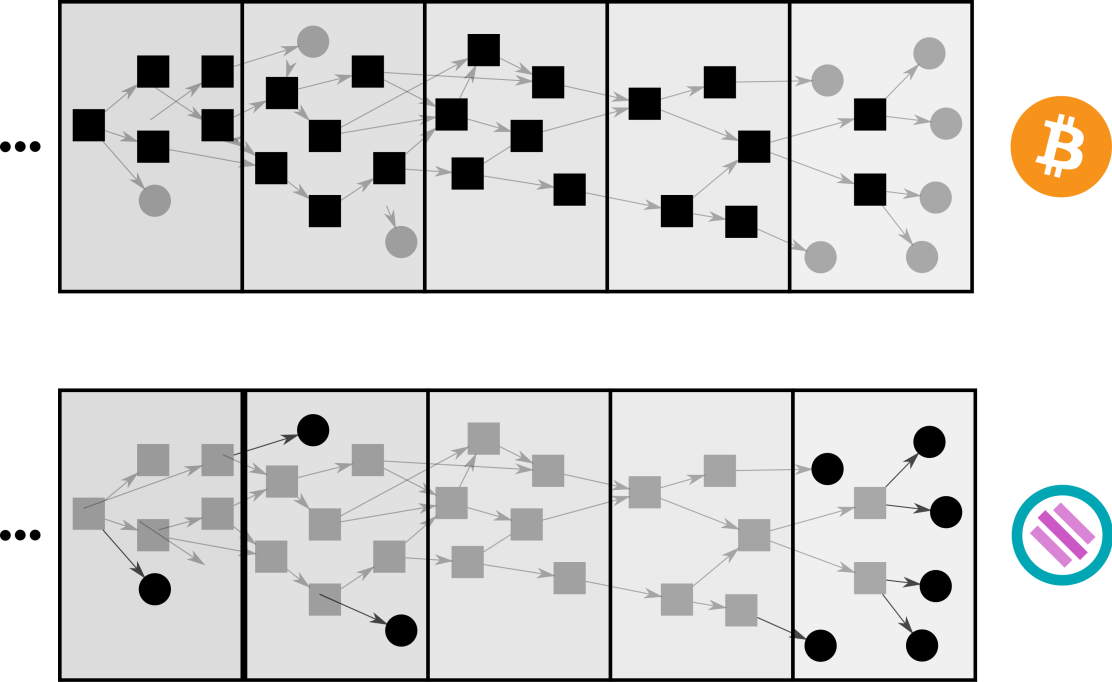
\includegraphics{../.gitbook/assets/coinint-eps-converted-to.png}
\caption{The ``worldview'' of a Bitcoin vs Themelio node}
\end{figure}

\hypertarget{consensus-and-trust}{%
\subsubsection{Consensus and trust }\label{consensus-and-trust}}

We now look at how nodes in Themelio come to agreement on the status of
the network --- decentralized \textbf{consensus}, the foundation of any
public blockchain's security. Themelio uses a variation of \emph{bonded
proof-of-stake} found in systems such as Tendermint. This is augmented
with a novel ``auditor'' system which further decentralizes trust.

\hypertarget{oligarchy-with-a-free-press}{%
\paragraph{Oligarchy with a free
press}\label{oligarchy-with-a-free-press}}

Participants in Themelio are divided into three categories by their
roles:

\begin{itemize}
\tightlist
\item
  \textbf{Stakeholder nodes} record transactions into new blocks and
  confirm them using a Byzantine fault-tolerant consensus algorithm
  between themselves. They communicate with each other through a
  broadcast protocol which other nodes in the network never participate
  in. Anybody can become a stakeholder by ``staking'' a cryptoasset.
  Stakeholders correspond to miners or validators in other systems.
\item
  \textbf{Auditor nodes} download newly created blocks from the
  stakeholders and gossip them between themselves while storing a local
  copy of the coin state. Anybody can join the network as a auditor by
  simply running a piece of software. Auditors verify new blocks decided
  by the stakeholders and check that the stakeholders never equivocate
  on the content of a given block height. Auditors roughly correspond to
  full nodes in other systems, although they have a more important role
  in Themelio's security.
\item
  \textbf{Client nodes} are lightweight participants that query the
  network of auditors to access specific information in the blockchain,
  yet do not trust any particular auditor.
\end{itemize}

From this overview we can already see that the trust model of Themelio
differs significantly both from that of traditional public blockchains
like Bitcoin and from that of typical private blockchains. This is one
of its major innovations. Themelio's trust can be summarized succinctly
as an \textbf{``oligarchy with a free press''}

\hypertarget{stakeholders-the-oligarchy}{%
\paragraph{Stakeholders: the
oligarchy}\label{stakeholders-the-oligarchy}}

\textbf{Synkletos: a new approach to proof-of-stake}

In Themelio, a Byzantine-resistant fault tolerant algorithm based on
HotStuff is used between the stakeholders to establish consensus on the
content of the blockchain. The stakeholders form an ``oligarchy'': most
users are not stakeholders, yet they get to decide the authoritative
state of the network. We call Themelio's consensus algorithm, together
with the cryptoeconomic mechanisms that keep stakeholders honest,
\textbf{Synkletos}, after the Greek name for the Byzantine Senate.

Synkletos keeps track of a special secondary currency on the blockchain
known as the \emph{sym}. Syms are traded freely alongside mels, the main
cryptocurrency of Themelio, with a regulated supply of 1 sym per block
(1.05 million syms per year). They can be thought of as ``shares'' in a
decentralized corporation in charge of deciding new blocks.

In order to become a stakeholder, one \emph{stakes} at least 1,000 syms,
locking them up for a fixed period of time (at least 500,000 blocks, or
approximately 6 months) as a performance bond. During that period of
time, the stakeholder obtains voting rights in the consensus algorithm
in proportion to the amount of syms staked. The central security
assumption Themelio uses is that \emph{at least 2/3 of the staked syms
are in the hands of honest stakeholders} --- a fundamental property of
Byzantine-fault-tolerant consensus means we can't get a better
threshold.

Two important questions remain:

\begin{itemize}
\tightlist
\item
  Why do we use proof of stake rather than another consensus mechanism?
\item
  How does Synkletos incentivize stakeholders to behave honestly, and
  what makes Synkletos' approach unique?
\end{itemize}

\textbf{Why proof-of-stake?}

Synkletos is a variation on \emph{proof of stake} (PoS), a family of
blockchain consensus algorithms including Tendermint and Casper. In
proof of stake, influence over the consensus process is in proportion to
owning an asset, in this case syms. Why did we choose PoS over other
consensus algorithms, such as the venerable proof of work (PoW) of
Bitcoin, or the proof of authority (PoA) found in consortium and private
chains? The Ethereum Proof-of-Stake FAQ {[}@buterin2019pos{]} give a
strong general defense of PoS; we highlight some properties of PoS we
consider especially important for Themelio:

\begin{itemize}
\tightlist
\item
  \textbf{Higher security margin}: Attacking a PoS blockchain directly
  requires expending an vast amount of resources to buy up stake. This
  is equivalent to around 1/3 of the total value of staking coins (a
  proxy of the economic value of the blockchain system). Thus, as usage
  increases, PoS security will proportionately strengthen until it
  becomes practically invulnerable to attacks on the consensus protocol.
  Proof-of-work blockchains like Bitcoin, however, can be subverted
  quite cheaply. Attacks reverting a full hour of Bitcoin transactions
  cost less than \$1,000,000 {[}@crypto51{]}, pocket change compared to
  the almost \$100 billion Bitcoin market capitalization. Finally, proof
  of authority, which is not a decentralized solution, is very fragile
  to centralized attack vectors such as hacking or government
  regulation.
\item
  \textbf{Immediate finality}: PoS allows easy, secure finality using
  asynchronous Byzantine fault-tolerant consensus protocols. This means
  that even if networks are unreliable or malicious, a block that is
  successfully appended to the blockchain will never be reverted. This
  eliminates the unpredictable behavior found in ``chain-based''
  consensus protocols like proof of work, such as forks, block
  reorganizations, and eclipse attacks.
\item
  \textbf{Stronger incentive-compatibility}: As we will see later,
  staked bonds allow us to punish misbehaving stakeholders by deleting
  their stake. In other blockchains, misbehaving miners only lose
  potential rewards or reputation. As the Ethereum FAQs put it, ``in
  PoW, we are working directly with the laws of physics. In PoS, we are
  able to design the protocol in such a way that it has the precise
  properties that we want - in short, we can optimize the laws of
  physics in our favor.''
\end{itemize}

\textbf{Rewards and slashing}

How do we incentivize stakeholders to behave honestly? We use a
carrot-and-stick approach commonly found in systems using bonded proof
of stake. Honest stakeholders earn \emph{rewards} over time in
proportion to the amount of syms they stake, while misbehaving
stakeholders can have their entire stake \emph{slashed} given evidence
of misbehavior.

Rewards to stakeholders come from two sources: \textbf{sym inflation}
and \textbf{transaction fees}. Stakeholders proposing new blocks earn
rewards of 1 newly minted sym per block, just like how Bitcoin miners
earn a fixed per-block reward. This implicitly taxes unstaked syms,
discouraging holding syms without staking them. Unlike in most other
blockchains, inflation is not intended to be the main source of
stakeholder income. Since we mint a fixed amount of syms every block,
the growth rate in the number of syms as well as the ``interest rate''
of staking syms approaches zero, making inflation significant only as a
short-term bootstrapping subsidy until fees reach a significant level.

Instead, \textbf{transaction fees} are used as the main source of
stakeholder revenue. Transaction fees, denominated in mels, are imposed
on every transaction on the network. Themelio uses a unique mechanism,
described in brief in the last section of this whitepaper, to charge a
slowly varying uniform fee voted on collectively by the stakeholders.
This mechanism, which is crucial to Synkletos' cryptoeconomic security,
allows fees to be a significant and stable source of income for
stakeholders, while avoiding well-known game-theoretical attacks such as
\href{https://www.cs.princeton.edu/~smattw/CKWN-CCS16.pdf}{fee-stealing}
associated with conventional auction-based fee markets.

\textbf{Slashing} is the ``stick'' for punishing cryptographically
provable misbehavior. The last step of our Byzantine-fault-tolerant
consensus protocol has all stakeholders \emph{commit} to a particular
block by signing it cryptographically. Honest stakeholders will always
commit a valid block and never ``go back'' on their collective decision.
Thus, we have two \emph{slashing conditions} which leave cryptographic
proof that a certain stakeholder is dishonest:

\begin{itemize}
\tightlist
\item
  \textbf{Equivocation}, where a stakeholder commits to two different
  blocks with the same block height
\item
  \textbf{Invalid block}, where a stakeholder commits to an invalid
  block
\end{itemize}

In either of these cases, anybody can submit cryptographic evidence (two
conflicting signatures, or a signature on an invalid block) as a
specially-formatted transaction on the blockchain. This \textbf{slashing
transaction} removes the offending stakeholder, deleting all of the syms
associated with the stake. Slashing also reduces the supply of syms and
increases the fraction of rewards that other stakeholders receive. This
incentivizes large stakeholders to monitor each other and slash
misbehaving stakeholders.

\textbf{Why two currencies?}

One of the unique features of Themelio's proof of stake is its separate
staking token, the sym, with features that intentionally discourage use
as money. Generally, PoS blockchains use their main ``money'' coin, like
ethers or EOS, as their staking asset. Why not do the same for Themelio?
Coins used as stake for consensus are fundamentally equity shares. They
are tokens representing fractional ownership of the transaction fees and
other ``profit'' of the system. Unfortunately, \emph{equity shares are a
poor form of money}.

First of all, for money we want flexible, demand-responsive monetary
policies to reduce value volatility. Otherwise, the currency becomes an
unpredictable store of value and a useless unit of account. In the
offline world, this is accomplished either by central bank policies for
fiat money, or natural supply elasticity for commodity money. For equity
shares though, unpredictable share dilution demolishes their fundamental
value proposition as fixed slices of profit. Thus, fixed minting
schedules, like those of bitcoins and syms, are perfect for equity, but
terrible for a new currency.

Furthermore, demand for equity shares in an efficient market is driven
largely by speculation on future cash flow, while demand for cash
derives from the need for a medium of exchange. We don't want users of a
currency to be forced to speculate on the future transaction fees of a
blockchain. Furthermore, increases in currency adoption as a means of
exchange shouldn't drive destabilizing bubbles in currency value.

Themelio therefore uses an independent currency, the \textbf{sym}, for
the role of equity stake. An independent equity token also turns out to
be crucial for establishing backing capital to stabilize the price of
mels, as detailed in the Melmint paper.

\textbf{Achieving high performance}

Scalable blockchains with immediate finality need a way to limit the
number of consensus participants. This is because Byzantine
fault-tolerant consensus algorithms have rapidly increasing overhead
with increasing participants. To achieve reasonable scalability and
performance, we are forced to limit the number of stakeholders to below
a few thousand.

Themelio's way of restricting the number of stakeholders is through the
minimum requirement of 1,000 syms staked per validator. Essentially, we
limit entry into the oligarchy of stakeholders to only the richest sym
holders. Since sym supply follows a fixed schedule, this places a hard
limit of a few hundred new validators a year, so that growth in overhead
won't outpace growth in computational capacity.

A large minimum stake seems, on the surface, unfair and unappealing.
After all, it ``disenfranchises'' the vast majority of potential
stakeholders and institutes a ``plutocracy''! Unfortunately, other
approaches that superficially sound more decentralized tend to have
crippling incentive problems. Ironically, they end up a lot more
vulnerable to centralized threats.

For example, a common method of deriving a small amount of participants
from a large body of coinholders is \emph{delegated proof of stake}
(DPoS). In DPoS, coinholders vote for people with voting power
proportional to their coin ownership, and only the few with the most
votes become ``delegates'' and participate in consensus. EOS is a
popular blockchain using DPoS.

Yet although DPoS gives a vote to all coinholders, it insulates
coinholders from protocol incentives. Coinholders are not responsible
for the actions of the delegates they vote for, while misbehaving
delegates receive no punishment other than a loss of reputation. Thus,
coinholders have no incentive to vote for ``good'' nodes, delegates have
little incentive to behave correctly, and misbehavior is rampant.
Unsurprisingly, all the problems of political governance in a
representative democracy get imported. Elections involve massive
advertising campaigns, vote-buying, and even nationalist agitation
{[}@zhihu2019votebuy{]}, while delegates often behave as a centralized
cartel, engaging in actions like censoring transactions
{[}@eoscensor{]}.

\emph{Sortition} is another approach, used most notably in Algorand
{[}@gilad2017algorand{]}. Periodically, a committee of participants is
randomly selected from all coinholders --- each coinholder has a
probability to win this ``lottery'' in proportion to the coins that they
hold. The committee then participates in a consensus protocol to decide
new blocks until the next lottery comes around.

Sortition eliminates most of the politics-like problems of DPoS,
allowing protocol incentives like rewards and slashing to work fairly
well. Unfortunately, severe problems remain. Randomly selecting
participants trustlessly turns out to be a surprisingly hard
cryptogrpahic problem --- a corrupt lottery can reliably elect malicious
committees. Bribery attacks also become much easier, since instead of
buying 1/3 of the coins, attackers can simply bribe the current
committee, who has only a small fraction of the stake. Complex consensus
protocols and advanced, non-quantum-resistant cryptographic techniques
can reduce both challenges. But ``fancy'' mechanisms generally go
against Themelio's philosophy of future-proof simplicity.

A point must be made that \emph{blockchain consensus is not analogous to
political governance}. Themelio's ``plutocratic oligarchy'' of
stakeholders certainly does not make for an effective way of electing a
parliament. But for blockchains, it yields highly robust and
decentralized security. It disperses control over blockchain consensus
to the few hundred people most invested in the health of the network. At
the same time, the Synkletos protocol keeps them correctly behaving with
massive carrots and sticks. Stakeholders do not decide political
questions for the Themelio community; their only job is to run the
consensus algorithm correctly.

Thus, we do not believe that Themelio's ``plutocratic'' bonded proof of
stake is any more vulnerable to centralized threats than PoS blockchains
without minimum stake amounts. Even so, Themelio has a system of
\emph{auditors} keeping stakeholders in check, ensuring that even a
fully corrupted quorum of stakeholders cannot do much damage.

\hypertarget{auditors-the-free-press}{%
\paragraph{Auditors: the free press}\label{auditors-the-free-press}}

\textbf{Making failure catastrophic}

The ``free press'' in Themelio consists of \emph{auditors}. Auditors are
``full nodes'' in usual terminology, replicating and validating the
entire blockchain. They form a random \emph{gossip} network among
themselves, similar to that used by Bitcoin full nodes. Through this
gossip network, information about new blocks is disseminated. Gossip
reduces load on the stakeholders and makes it difficult for malicious
networks to censor the blockchain --- as long as some auditors can
connect to the stakeholders and the auditors form a connected graph, new
blocks will quickly be visible to every auditor.

The more important role of auditors, though, is to \emph{make consensus
failure catastrophic}. This plays a crucial role in keeping the
oligarchy of stakeholders honest. Auditors utilize their position as
relayers of new blocks to continually monitor for evidence that the
stakeholder consensus is corrupt. For example, invalid blocks or two
different blocks at the same height signed by a quorum would be proof
that the coordinators are no longer trustworthy. These pieces of
evidence, known as \emph{consensus nukes}, undeniably prove that at
least 1/3 of the stakeholders are actively malicious or compromised.

Any auditor that sees a consensus nuke immediately broadcasts it to all
auditors it knows in the gossip network. It then permanently activates a
``kill switch'' and refuses to operate normally. Thus, an attempt at
forking or appending invalid transactions to the blockchain would
figuratively "nuke" the entire network.

\textbf{Why consensus nukes?}

This objective seems a little strange. Why would we ever want our
network to self-destruct?

The obvious answer is that if we no longer have a 2/3 supermajority of
honest stake, the entire system is irrecoverable. More specifically, a
well-known result {[}@dwork1988consensus{]} mathematically proves that
consensus protocols running in a partially synchronous network model
(that is, network delays are unknown but finite) cannot possibly
tolerate more than 1/3 arbitrary faults. So we have to choose between a
model where the network stays up, but malicious stakeholders can corrupt
the state arbitrarily (rewriting history, giving themselves free money
--- or shutting down the network), or one where the only thing a
corrupted quorum can do is shut down the network. Clearly, the latter is
preferable.

More importantly, consensus nuking changes the incentives of potential
attackers by making most attacks unprofitable. Consider a blockchain
where consensus-breaking attacks (like Bitcoin's 51\% attack) allow
arbitrary state corruption. A malicious actor with the ability to
execute such attacks can extract huge profits simply through
double-spending. With more complex higher-level applications relying on
blockchain data, profit opportunities are even more numerous. Thus, if
enough rationally self-serving stakeholders collude, they are greatly
incentivized to attack the network and destroy its security guarantees.

If a successful attack can only result in the network stopping all work,
only attackers who benefit from destroying the network will participate.
Since a successful attacker must stake a vast amount of syms to take
over more than 1/3 of the stake, destroying the network and thus the
value of the investment is usually irrational.

Finally, a shutdown when a successful attack occurs forces Themelio
users to manually coordinate an emergency ``hard fork'' out-of-band to
restore the network. This would involve, at the very least, a
redistribution of stakes away from the attacking parties and possibly
protocol improvements to prevent future attacks. On the other hand, if
the blockchain continues to operate even when stakeholders are
corrupting the state, nothing forces users to coordinate a hard fork.
It's conceivable that the malicious stakeholder cartel can create a
climate of pressure for users to go along with the corrupted chain ---
for example, the state corruption might be forced by legal regulation or
presented as way of restoring stolen assets. Consensus nuking ensures
that these scenarios are impossible.

\hypertarget{clients-thin-yet-fully-secure}{%
\paragraph{Clients: thin yet fully
secure}\label{clients-thin-yet-fully-secure}}

Most users of a blockchain, Themelio not excepted, do not have nearly
enough resources to process all transactions 24/7. Users that do not
synchronize the whole blockchain state, known as thin clients, serve a
vital role in any blockchain system. In other blockchains, though, thin
clients come with both reduced security and mediocre performance.
Bitcoin, for example, has thin clients who must persistently store a
growing set of block headers and connect to at least one trusted full
node.

In Themelio, thin clients (usually just called clients) are both thinner
and safer than thin clients in other systems. Clients only synchronize a
small piece of data, less than a kilobyte in size, a few times a year.
Yet with this data, they can fully validate a large variety of
information they can freely obtain from auditors. Even if a client only
connects to bad auditors, it cannot be fooled into accepting invalid
data. We accomplish this through two technical innovations:
\emph{metastate commitments} in block headers and \emph{epoch-based
stake bonds}.

\textbf{Metastate commitments}

Blocks in Themelio, like those in almost all blockchains, have
constant-size \emph{headers} that summarize information about that
block. Block headers typically cryptographically \emph{commit} to
certain pieces of information, such as the transactions within a block,
through hash trees and similar mechanisms. Cryptographic commitments
allow thin clients to verify claims about the data they commit to
without trusting third parties or downloading the entire blockchain.

In traditional coin-based blockchains, block headers commit only to the
previous block header and the transactions within the block. This means
thin clients can only verify claims that a certain transaction occurred
in a block --- this is not enough even for basic applications like
wallets to be trustless. Account-based blockchains like Ethereum improve
on this by committing to the \emph{state}, or all the information needed
to validate new transactions. This allows apps like wallets that rely on
querying the state to run trustlessly.

In Themelio, the state is simply the set of all unspent coins. We use a
sparse Merkle tree to commit in the block header to a mapping of the
coin identifier (hash of the transaction that produced the coin and
index of the coin) to coin metadata (value, constraint, etc). This
allows thin clients to verify whether or not a coin is spent at a
certain block height.

For some simple applications, like verifying a Catena log, this is
sufficient. Unfortunately, many applications on coin-based blockchains
need to access more than the plain state mapping. For example, wallets
would want to know which coins to spend without proofs of payment from
all incoming payers.

We therefore commit not just to the state mapping, but also to
\emph{metastate}, or metadata about state. Metastate is not strictly
necessary for validating blocks, but cryptographic commitments to it in
the block header allows more powerful thin clients. This includes
information like:

\begin{itemize}
\tightlist
\item
  Number of unspent coins with a certain constraint
\item
  Total number of transactions in the block
\item
  Current block height
\end{itemize}

Thus, complex coin-oriented applications can trustlessly run on clients
that don't need to synchronize anything but the latest block header.

\textbf{Epoch-based stake bonds}

One problem remains: how are clients supposed to get the latest block
header? In many blockchains, clients simply synchronize \emph{all} the
block headers. Clients would thus use ``proof-of-consensus'' information
(in Bitcoin's case proof of work) embedded in each header to verify the
next.

In Themelio, such a strategy would be prohibitively expensive. One of
the tradeoffs we made that allows robust proof-of-stake immune to
network problems is greatly increased sizes of proofs of consensus. A
proof that a block header belongs to the valid blockchain in Themelio
requires cryptographic signatures from at least 2/3 of the stakeholders
--- about 10 KB for a reasonable number of stakeholders. Furthermore,
there are just a lot more blocks in Themelio than in Bitcoin. Instead of
blocks 10 minutes apart, Themelio produces a block every 30 seconds.
This means that in just a year, the block header consensus proofs would
amount to more than 10 GB.

To fix this problem, Themelio divides blocks into \emph{epochs} lasting
500,000 blocks, or about half a year. Within each epoch, the list of
shareholders and their respective voting weights stays the same. All
stake-related transactions, such as staking and slashing, take effect
only at the start of the next epoch. Finally, the last block header of
each epoch embeds a \emph{stake document}, which includes the
shareholders and voting weights to use when validating blocks in the
next epoch.

This means that to validate, say, block header 1,100,000, we simply need
the stake document embedded in block 999,999. And to validate that stake
document, we just use the stake document in block 499,999. This process
repeats until we get to a stake document we already know about.

So clients simply have to catch up on all the new stake documents they
missed --- 10 KB every 6 months. Afterwards, they can securely validate
the latest block header, which then lets them check claims about almost
any fact about coins. Such ultra-thin clients allow apps using Themelio
to scale on small devices like smartphones, while keeping trust totally
decentralized.

\hypertarget{cryptocurrency-and-economics}{%
\subsubsection{Cryptocurrency and
economics}\label{cryptocurrency-and-economics}}

Finally, we examine the cryptocurrency economy of Themelio, based on a
low-volatility currency called the \textbf{mel}.

\hypertarget{mels-an-endogenous-stablecoin}{%
\paragraph{Mels: an endogenous stablecoin
}\label{mels-an-endogenous-stablecoin}}

Mels are optimized to be the day-to-day transaction currency on
Themelio. One can imagine decentralized apps, grocery stores, and
peer-to-peer finance to conduct transactions mainly denominated in mel.

The biggest feature of the mel is that it is an \textbf{endogenous
stablecoin}. This is a completely novel asset class introduced by
Themelio, and it means that the mel maintains a stable value without
being pegged to any external asset, such as US dollars or gold. Mels
maintain their value without non-endogenously-trusted parties present in
every other stablecoin system, such as oracles, governance DAOs, and
issuers.

The ``magic'' behind mel through a currency issuance algorithm we
published at
\href{https://assets.pubpub.org/1tfwdfex/01581339020290.pdf}{CryptoEconSys
2020} called Melmint. The details are available in the paper, but the
basic objective of Melmint is to peg the value of 1 mel to 1 ``DOSC'', a
unit that tracks the cost of 24 hours of sequential computation.

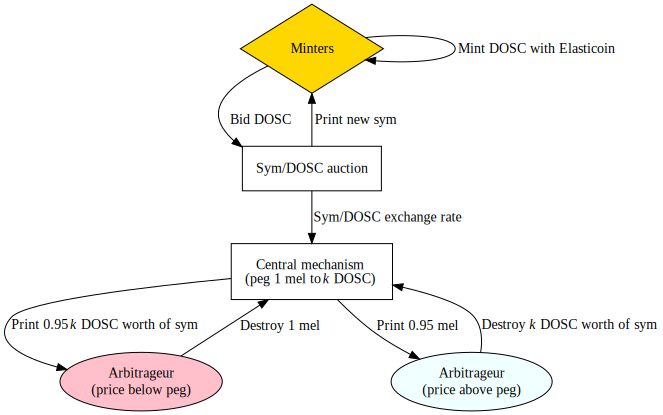
\includegraphics{../.gitbook/assets/graphviz-2-.svg}

By having a stable purchasing power without sacrificing trust, mels
would make it much easier to build secure financial assets, transact in
cryptocurrency, and protect wealth with Themelio's endogenous trust.

\hypertarget{better-transaction-fees}{%
\paragraph{Better transaction fees}\label{better-transaction-fees}}

As in Bitcoin and other public blockchains, each transaction in Themelio
includes a transaction fee to compensate stakeholders and make flooding
attacks costly. Most other blockchains let transaction senders
voluntarily decide whatever fee they like; block creators then decide
which transactions to include in the limited space within a block. This
functions as a pretty fair and efficient first-price auction, since
transactions with more fees relative to the burden they pose to the
network get higher priority. Unfortunately, auction-based transaction
fees paid to whoever included the transaction in a block have several
significant problems:

\begin{itemize}
\tightlist
\item
  \textbf{Fees are extremely volatile}. When blocks are filled, average
  fees will vary quite a lot as demand fluctuates. In practice,
  persistently full blocks is the norm, whether due to demand increase
  in protocols like Bitcoin where the block size cap is fixed, or due to
  block producers setting block limits according to demand as in
  Ethereum. Thus, fees for full blocks are extremely volatile in
  existing blockchains, often changing as much as 2x within one block
  interval. This makes for a very poor user experience.
\item
  \textbf{Complex client-side fee estimation}. It's far from trivial how
  much fees to bid in order to get transactions confirmed in a
  traditional fee market. Wallets need complicated algorithms to
  estimate the right amount of fee based on looking at unconfirmed
  transactions --- which thin clients can't even securely monitor.
\item
  \textbf{Stakeholder incentive problems}. In a proof-of-stake system
  like Themelio, we want stakeholder income to come primarily from
  transaction fees. That way, stakes have values in proportion to the
  value of the system, making attacks harder as usage grows (and damage
  increases), while giving stakeholders a disincentive to collude to run
  Themelio into the ground. But a conventional fee market encourages
  stakeholders to hide transactions from each other --- a transaction
  you include in a block is a transaction fee that I didn't get ---
  leading to all sorts of pathological ``fee-stealing'' strategies
  unless stakeholders have a different source of income. This is why
  Bitcoin and Ethereum rely heavily on inflation, not fees, to reward
  block producers, but we don't want that in Themelio.
\end{itemize}

Thus, we abandon the traditional fee auction model in favor of a system
inspired by EIP-1559 {[}@eip1559{]}, which also turns out to be crucial
for Synkletos' security. Every transaction pays a mel-denominated fee
that has two components. A mandatory \emph{base fee} is calculated by
multiplying by the \emph{base fee multiplier} the \emph{weight} of a
transaction, a metric that roughly measures its cost. Transaction
senders can then add a \emph{tip} above and beyond the base fee.

Every time a new block is created, the stakeholder proposing the block
can adjust the base fee multiplier by up to 1\% upwards or downwards ---
the base fee multiplier then reflects the stake-weighted median of the
stakeholders' preferences. Base fees, except for an eighth which is
burned, are deposited into a special \emph{fee pool} regardless of who
included the transaction into the blockchain; the stakeholder creating a
block then withdraws a tiny fraction (\(1/65536\)) of the fee pool. The
net effect is that the base fee of a transaction is distributed to all
stakeholders regardless of who made the block that contains the
transaction.

Tips, on the other hand, are simply paid to the block producer, like
fees in traditional blockchains. We expect tips to be a small fraction
of total fees, and they give an incentive for block producers to
actually include transactions instead of freeloading on a fee pool
replenished by other, more honest block producers.

Why do our changes to the fee market fix its problems? First of all, fee
volatility is greatly reduced. When demand fluctuates in the short term,
it would be block sizes that fluctuate, not fees. Stakeholders adjust
the base fee multiplier to maximize revenue and limit block sizes, but
not rigidly at a defined size. One might object that stakeholders can
collude to recreate Bitcoin's fee market --- by holding down the
multiplier to zero, enforcing an unofficial block size limit, and
auctioning off block space based on tips. But a rational stakeholder
cartel will not do so, as assuming no change in demand, this will simply
greatly increase income volatility without increasing expected total
income, while in reality volatile fees will probably scare away some
users, actually reducing revenue. Incidentally, this is also why we
award base fees to stakeholders rather than burning them as in EIP-1559,
since burning base fees will make colluding to create a fee aucion
highly profitable.

Secondly, clients no longer need complex algorithms to compute fees. The
base fee plus a small tip will be sufficient in all cases to get a
transaction onto the blockchain as fast as possible. Applications like
wallets or payment processors would easily predict the amount of fees
needed.

Finally, although we still reward stakeholders with some sym inflation
to bootstrap network growth, the use of a fee pool ensures that even
though stakeholders are rewarded mostly from fees, there's no incentive
to steal fees. In fact, one can think of the fee pool as a sort of
long-term trust fund, derived from fees, for a stable Bitcoin-like block
reward.

\hypertarget{applications-and-protocols}{%
\subsection{Applications and
protocols}\label{applications-and-protocols}}

Let's now take a look at the sort of protocol and application ecosystem
that Themelio supports. Current patterns for blockchain application
development are often unsuitable for Themelio due to the lack of
features such as smart contracts and sharding. We start from simple to
complicated apps, showing how with the help of novel upper-layer
abstractions and protocols, decentralization be much more robust and
performant.

\hypertarget{astramel-scalable-payments}{%
\subsubsection{Astramel: scalable
payments}\label{astramel-scalable-payments}}

Obviously, on-chain mel transactions can be used directly to send money.
However, as Themelio only processes at most 1000 transactions a second,
this does not scale to the extent required for global microtransactions.

Fortunately, a solution already exists: payment channels. Payment
channels networks, used in protocols like Lightning Network on Bitcoin
or Raiden on Ethereum, route secure cryptocurrency payments through
untrusted intermediaries, allowing fully trustless payments without
conducting every transaction on the blockchain. PCNs are in fact a
primary example of a largely \emph{logically decentralized} protocol
with no consistent global state --- they work very similarly to the
mutual-credit networks underpinning money transfers in the banking
system --- yet they derive their security ultimately by relying on the
logically centralized blockchain as a root of trust.

Existing payment channel constructions for coin-based blockchains, like
the Poon-Dryja channels used in Lightning Network, can easily be ported
to Themelio. Perhaps more importantly, MelScript allows powerful
bidirectional payment channels to be constructed in a straightforward
manner without hacks such as the temporary keypairs used in Poon-Dryja
channels.

Compared to payment channel networks on blockchains like Bitcoin or
Ethereum, a Themelio PCN would provide far better scalability simply due
to the faster blockchain --- after all, opening and closing payment
channels is still limited by blockchain throughput. And compared to the
traditional banking network, payment channels give immediate trustless
finality, without any authorities that can steal funds or reverse
payments. Even on the scalability side, a payment channel network on
Themelio will greatly outperform traditional methods in volume and
latency, allowing custodian-free microtransactions for applciations like
paying road tolls.

We have already developed Astrape, a novel PCN construction that
achieves both competitive performance and very strong anonymity. A
variant of Astrape, Astramel, is under development as a Themelio project
to become a standardized scalable asset-transfer scheme for the Themelio
blockchain.

In fact, we intend Astramel to be the primary payment protocol for
Themelio, rather than raw on-chain transactions. Even for a ``basic''
functionality like value transfer, we believe that an indefinitely
scalable, logically decentralized protocol should be the standard.

\hypertarget{conifer-and-bitforest-trust-minimizing-naming}{%
\subsubsection{Conifer and Bitforest: trust-minimizing
naming}\label{conifer-and-bitforest-trust-minimizing-naming}}

Using blockchains to implement decentralized and secure naming systems
is not a new use case. Blockstack and ENS are examples of
blockchain-backed naming systems, which consistently map human-readable
identifiers (such as domain names) to security-critical information like
public keys without trusting third parties. Legacy naming systems, like
DNS and CA-based PKI, are highly centralized and have very fragile
security, so even for traditional centralized services like websites, a
blockchain-backed, easily deployable naming system can significantly
improve security.

It's not obvious how to embed a naming system in a coin-based blockchain
like Themelio. We have developed and published two naaming protocols
with different design tradeoffs, Conifer {[}@dong2018conifer{]} and
Bitforest {[}@dong2018bitforest{]}, for coin-based blockchains. Both
encode name bindings as a combination of an on-chain transaction graph
and off-chain centralized servers. Notably, both Conifer and Bitforest
are \emph{federated} naming systems similar to DNS, where names are
issued by diverse authorities, but both use the logically centralized
trusted functionality of a blockchain to ensure that such authorities
cannot engage in attacks such as impersonation and equivocation.

Themelio's more powerful coin-based programming paradigm is especially
suited for implementing these transaction graph-based naming systems.
Notably, by using MelScript instead of simple authority-controlled
signature scripts, we can enforce invariants in on-chain transaction
graphs without the name-issuing authorities used in Conifer and
Bitforest. This allows us to develop variants of Conifer and Bitforest
that are entirely decentralized, using technologies such as DHTs to
implement the logically decentralized part of the naming system.

Compared to existing blockchain solutions, a Themelio-based naming
system would offer higher performance due to the blockchain's higher
throughput, but much more importantly, a paradigm that encourages
extensive use of horizontally-scaling off-chain decentralized protocols.
Furthermore, Themelio's powerful thin-client abilities allow deploying
blockchain-based naming directly to the smallest of edge devices, rather
than relying on trusted gateways like in Blockstack. This removes one of
the biggest challenges in deploying naming systems with fully
decentralized trust.

\hypertarget{token-systems}{%
\subsubsection{Token systems}\label{token-systems}}

Another major use case for Themelio is for tokens, like fundraising
tokens, cryptokitties, and new cryptocurrencies. Right now, a token is
most commonly implemented as a big stateful smart contract on Ethereum,
following API standards like ERC-20. This way of implementing a token,
unfortunately, is prone to error, often leading to critical security
vulnerabilities. Scalability is also a big challenge, as massive
stateful smart contracts cannot be easily parallelized even with
advanced features like sharding.

In Themelio, on the other hand, custom tokens are ridiculously easy to
create. Themelio tokens rely on a special case in its transaction
verification logic. Transactions must be balanced by currency --- the
total values of mels, syms, etc in the input coins spent must be equal
to the total values in the outputs --- with the exception that an
unlimited number of coins, with unconstrained values, can be created
with \emph{unlabeled} units. Outputs with unlabeled units will then
create coins in the blockchain state with a new unit derived from the
unique ID of the transaction.

Thus, a new cryptocurrency token can be created simply by creating any
regular transaction while tacking on an additional unlabeled output with
the value set to the maximum supply of the new token. This coin's
constraint script will then determine the rules of token issuance --- no
other transactions can create coins with the same unit, since custom
tokens are always denominated by the first transaction that created
them.

As an example, imagine Foobar wants to create a new token, FooCoin.
FooCoin would be sold to the public at a fixed rate of 1000 nanomels per
coin. Foobar would broadcast a transaction, say with ID
\texttt{0xdeadbeef}, with an unlabeled output with an inexhaustibly
large value (say \(2^{64}\)) and the following constraint:

\begin{verbatim}
;; first output sends the rest of the FooCoins
;;   and repeats this constraint
;; second output sends FooCoin to buyer
;; third output sends mels to Foobar
(and (output-like? 0
      #:currency 0xdeadbeef
      #:constraint (output-constraint *SELF*))
     (output-like? 1
      #:currency 0xdeadbeef)
     (output-like? 2
      #:currency 'nTMEL
      #:constraint FOOBAR
      #:value (* (output-value (output-ref 0))
                  1000)))
\end{verbatim}

Anybody can then spend this FooCoin-denominated output, diverting some
of the FooCoin to himself, leaving the rest with the same constraint,
and giving FooBar mels in compensation. FooCoins not encumbered by this
constraint freely transact using the same rules as syms and mels do,
with no complex smart contracts needed to handle all the cases. Wallet
software, payment processors, etc can simply check for coins denominated
in ``\texttt{0xdeadbeef}'' to support FooCoins.

Analogous constraints can be used to implement more complex rules for
fungible cryptocurrency tokens. Non-fungible tokens are implemented
simply by creating an a new token unit with a coin that has a value of
1. Since 1 cannot be further subdivided, this means that only one coin
of that token can ever exist.

\hypertarget{autonomous-applications}{%
\subsubsection{Autonomous applications}\label{autonomous-applications}}

The vast majority of Ethereum-style smart contracts deal with
``asset-like'' objects like tokens and names and can usually be
translated into a simpler and more robust coin-based version on
Themelio. One proposed category of decentralized app, though, typically
requires a vast amount of state tracking and complex logic and is hard
to implement directly on Themelio --- ownerless, fully autonomous
applications. For example, a smart contract on Ethereum might be an
autonomous financial company, negotiating legal contracts, generating
packaging its assets into financial products, and pay the bills for a
marketing website while hiring people to maintain it, all without human
intervention.

Autonomous blockchain entities as described do not really exist except
as a concept, and in any case such programs would not be able to scale
on Ethereum and other present blockchains due to their poor performance.
An autonomous application with security rooted on Themelio would have to
implement most of its logic outside the blockchain even if Themelio
could provide the requisite performance. For example, the autonomous
financial company might run its business logic on traditional cloud
services, while accepting payment and paying for its own bills with mels
and issuing Themelio-based financial assets. This way, the program would
not spam the blockchain with transactions every time its internal state
changes. Trustless operation can be achieved by synchronizing state
through a trustless private blockchain, as described in the next
section.

\hypertarget{trustless-private-blockchains}{%
\subsubsection{Trustless private
blockchains}\label{trustless-private-blockchains}}

For some applications, nothing short of a new blockchain with its own
would do. Traditionally, this would require deploying a new blockchain,
private or public, just for use within the application. But this greatly
reduces security, as compromising a blockchain formed by consensus
between a small number of people is much easier than taking over a
public blockchain like Themelio or Ethereum.

One solution is to use a \emph{metachain}, also known as a
\emph{virtualchain}, where every time a transaction happens on the
smaller blockchain, it is embedded into a corresponding transaction on a
public blockchain. Clients of the metachain then scan the entire public
blockchain for valid-looking transactions to reach a consensus on the
state of the metachain --- a very slow process.

Metachains can, of course, be implemented on Themelio, but using
Themelio's more expressive features can greatly increase their
performance. For example, all transactions claiming to be part of the
metachain can be placed in a permissionless Catena log (see
\href{}{2.2.3}). Metachain clients could then avoid scanning through the
mass of unrelated Themelio transactions.

If the state transition function of the metachain can be expressed in a
short MelScript constraint, Themelio could even enforce the rules of the
metachain. This can be combined with using a unique ``non-fungible
token'' inside the Catena log to label the metachain. That way, any thin
client can request the transaction with the one and only unspent output
denominated in that token, and that transaction is guaranteed to contain
the latest state of the metachain.

As described, metachains would be public and permissionless, but similar
techniques can be used to secure private blockchains. Data in metachains
can be encrypted with a key that only authorized parties know, and the
Catena log can have a signature-checking constraint to block
unauthorized users from spamming the metachain. Permissioned metachains
have a very attractive combination --- they inherit the immutability and
trustlessness of Themelio, while preventing public access to the
contents of the metachain. We believe this is a much better fit for
business appliations like bid tendering or supply-chain tracking than
private or consortium blockchains.

\hypertarget{conclusion}{%
\subsection{Conclusion}\label{conclusion}}

Public blockchains, as originally envisioned, herald a fundamental
revolution in the way trust works in distributed systems. Unfortunately,
they have not seen widespread usage in production systems, outside of a
few applications using private blockchains that eschew most of
blockchains' distinctiveness. Blockchain development has also run into
many serious obstacles, such as scalability and governance.

In this whitepaper, we argued that the main reason for the seeming
failure of public blockchains is an incorrect layering paradigm ---
current blockchains are generally too close to the application layer,
forcing complex blockchain implementations on one hand and ``leaky'',
rigid applications on the other hand. We propose that the correct
paradigm for blockchains is that of a minimal root of trust, providing a
magic ingredient of endogenous trust to applications that mostly run
outside the blockchain.

We described Themelio, a blockchain we developed to support this vision,
using many novel technologies and design tradeoffs not seen in current
blockchains. We also illustrated the wide range of applications that can
be developed using Themelio within a blockchain-minimizing paradigm.

\end{document}
